%%%%%%%%%%%%%%%%%%%%%%%%%%%%%%%%%%%%%%%%%
% Beamer Presentation
% LaTeX Template
% Version 1.0 (10/11/12)
%
% This template has been downloaded from:
% http://www.LaTeXTemplates.com
%
% License:
% CC BY-NC-SA 3.0 (http://creativecommons.org/licenses/by-nc-sa/3.0/)
%
%%%%%%%%%%%%%%%%%%%%%%%%%%%%%%%%%%%%%%%%%

%----------------------------------------------------------------------------------------
%	PACKAGES AND THEMES
%----------------------------------------------------------------------------------------

\documentclass{beamer}
\mode<presentation> {

% The Beamer class comes with a number of default slide themes
% which change the colors and layouts of slides. Below this is a list
% of all the themes, uncomment each in turn to see what they look like.

%\usetheme{default}
%\usetheme{AnnArbor}
% %\usetheme{Antibes}
%\usetheme{Bergen}
%\usetheme{Berkeley}
%\usetheme{Berlin}
%\usetheme{Boadilla}
%\usetheme{CambridgeUS}
%\usetheme{Copenhagen}
%\usetheme{Darmstadt}
%\usetheme{Dresden}
%\usetheme{Frankfurt}
%\usetheme{Goettingen}
%\usetheme{Hannover}
%\usetheme{Ilmenau}
%\usetheme{JuanLesPins}
%\usetheme{Luebeck}
\usetheme{Madrid} %%%%
%\usetheme{Malmoe}
\setbeamertemplate{navigation symbols}{} % To remove the navigation symbols from the bottom of all slides uncomment this line
\setbeamertemplate{itemize items}[default]
\setbeamertemplate{enumerate items}[default]

\definecolor{UDMblue}{RGB}{46,78,161}
\setbeamercolor{structure}{fg=UDMblue}
%\setbeamercolor*{item}{fg=red}

}



\usepackage{graphicx} % Allows including images
\usepackage{graphics}
\usepackage{booktabs} % Allows the use of \toprule, \midrule and \bottomrule in tables
\usepackage[english, french]{babel}  %support francais et anglais
\usepackage[utf8]{inputenc}
\usepackage{subfig}
\usepackage{caption}
%\usepackage{subcaption}
\usepackage{setspace}

%\usepackage{ marvosym }
%\usecolortheme{orchid}
%\setbeamercolor{alerted text}{fg=white}
%\usecolortheme{default}

%\usecolortheme{default}
%\graphicspath{{./figures/}}
\begin{document}

\pgfdeclareimage[width=10cm]{logos_criugm}{logos_criugm}
\title[Mining brain networks]{Neuroimaging Analysis Kit - Overview}
\author[NIAK team]{NIAK development team \\ \tiny{\texttt{niak.simexp-lab.org}}}
%\institute[BIC]{\vspace{-0.2cm}}
\date[]{\pgfuseimage{logos_criugm} }


\frame{\titlepage}

\section{NIAK fMRI preprocessing pipeline}

{
\usebackgroundtemplate{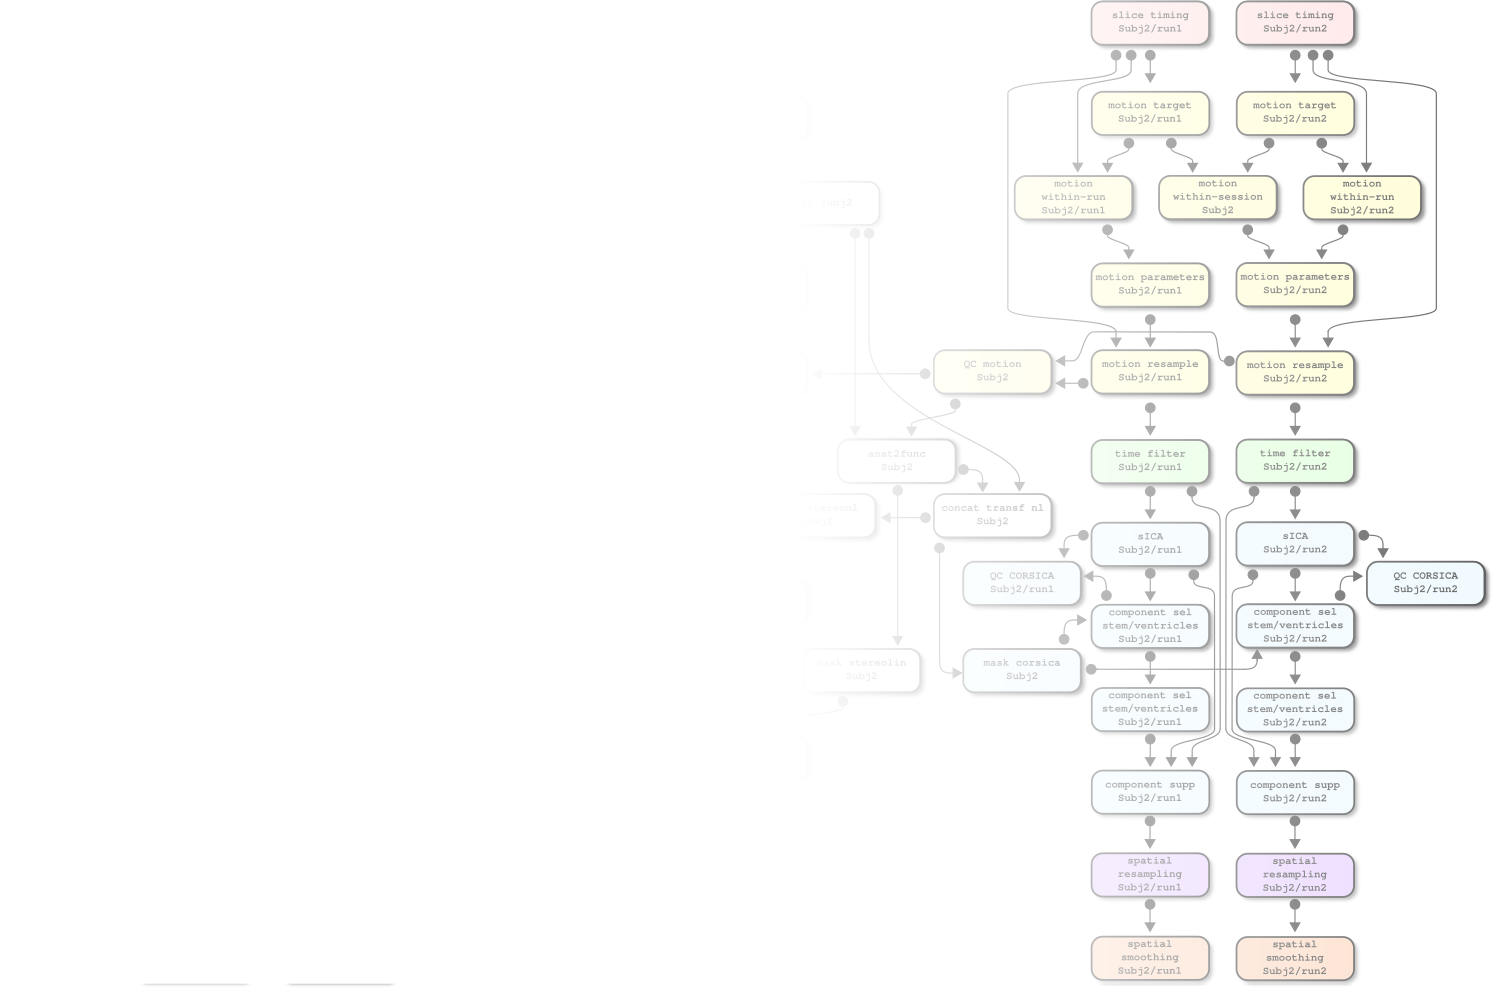
\includegraphics[height=\paperheight]{fig_pipelines.png}}

\frame{
\frametitle{What's NIAK}
The Neuroimaging Analysis Kit (NIAK): \\
a software package for connectivity analysis\\
in large fMRI datasets.
\begin{itemize}
\item A catalogue of \textbf{complete workflows}.
\item \textbf{Scales} for large datasets / analyses.
\item \textbf{Reproducible} deployment. 
\item \textbf{Well tested} workflows. 
\item Web-based \textbf{notebook} interface.
\item Interactive \textbf{dashboard} reports.
\item Free and \textbf{open-source} (MIT).
\end{itemize}
}
}

{
\usebackgroundtemplate{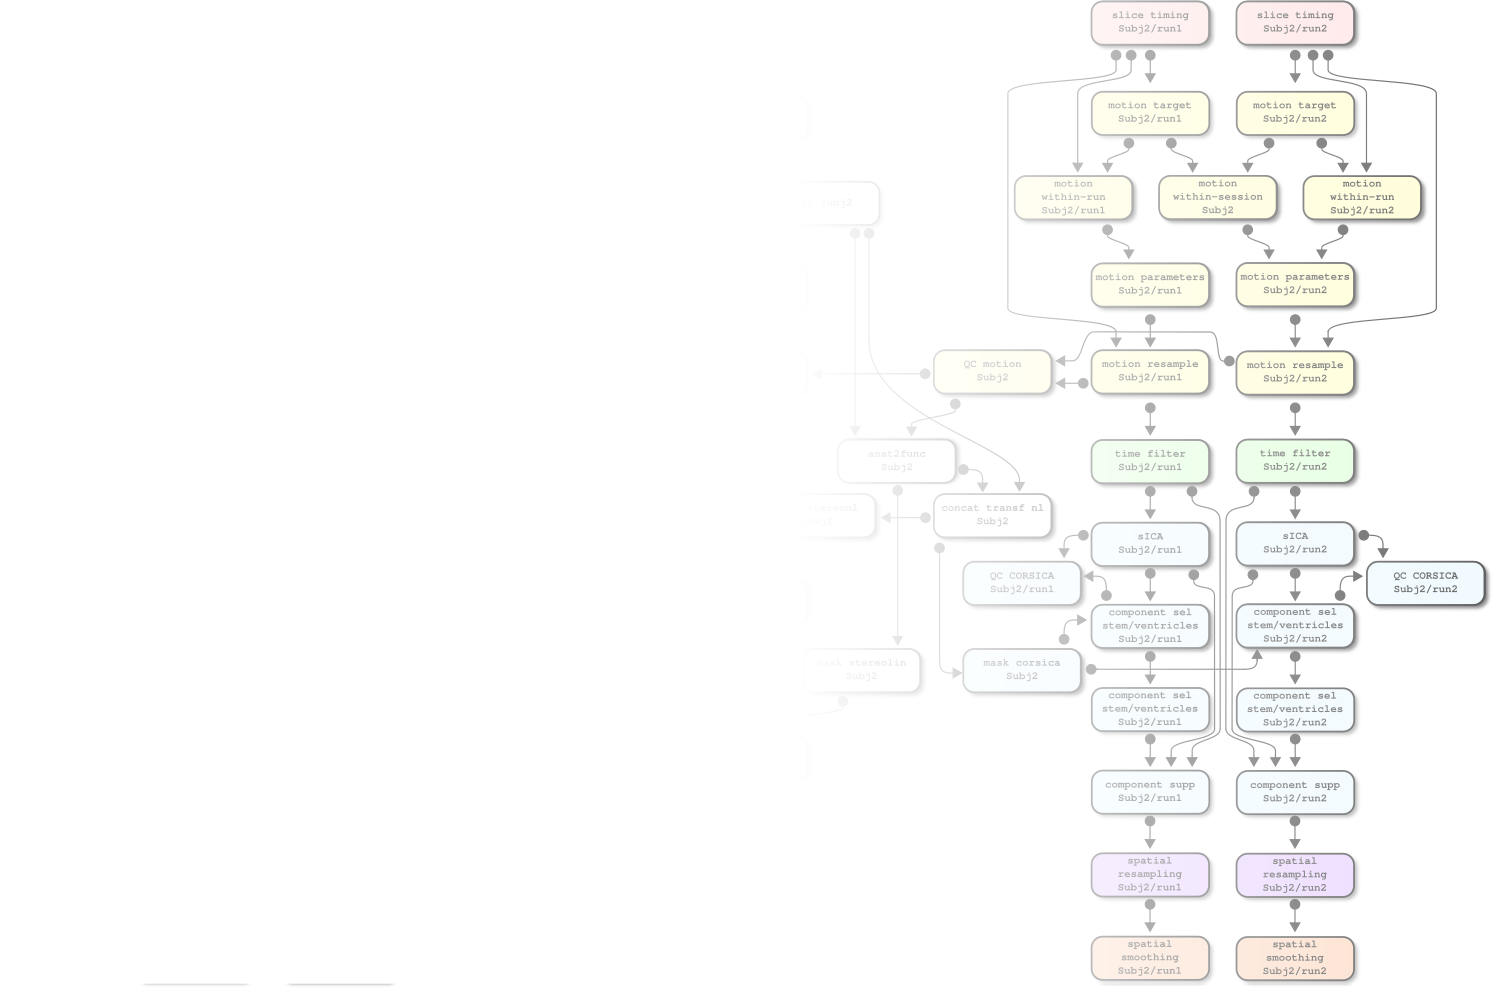
\includegraphics[height=\paperheight]{fig_pipelines.png}}

\frame{
\frametitle{Available pipelines}
\begin{center}
\begin{figure}
\pgfimage[width=0.8\linewidth]{fig_summary_niak}\\
\end{figure}
\end{center}
Check \url{http://niak.simexp-lab.org} for more info.
}
}

\frame{
\frametitle{Main dependencies}
\begin{itemize}
 \item \textbf{Ubuntu}: An operating system based on mostly GNU tools as well as the linux kernel. Free software (mixed licenses). \url{https://www.ubuntu.com/}
 \item \textbf{Octave}: A high-level scientific programming language, largely identical to Matlab. Octave is Free Software (GNU license). \url{https://www.gnu.org/software/octave/} 
 \item \textbf{The MINC toolkit}: A set of command line tools for brain registration, segmentation and basic image processing operation. Underlying code is mostly C and PERL. Free sotware (MIT like custom license). \url{http://bic-mni.github.io/} 
 \item \textbf{The brain connectivity toolbox}: A toolbox to generate properties of brain networks. \url{https://sites.google.com/site/bctnet/}.
 \end{itemize} 
}

\section{High-performance computing}

\frame[containsverbatim]{
\frametitle[report]{One pipeline, many jobs...}
\centering

\pgfimage[width=0.9\linewidth]{fig_dep_fmri_preproc}\\
\centering
\tiny Jobs and dependencies for fMRI preprocessing of two subjects with two functional runs each.
}

\frame[containsverbatim]{
\frametitle[What's PSOM?]{The pipeline system for Octave and Matlab}
NIAK is powered by PSOM, an open-source library for scripting pipelines using Octave or
Matlab (Bellec et al., Frontiers in Neuroinformatics, 2012).
\begin{itemize}
 \item \textbf{Parallel computing}: Detection and execution of parallel components in the pipeline. The same code can run in a variety of execution environments (local, multi-core, cluster). 
\item \textbf{Provenance tracking}: Generation of a comprehensive record of the pipeline stages and the history of execution. 
\item \textbf{Fault tolerance}: Multiple attempts will be made to run each job before it is considered as failed. Failed jobs can be automatically re-started. 
\item \textbf{Smart updates}: When an analysis is started multiple times, only the parts of the pipeline that need to be reprocessed are executed. 
 \end{itemize} 
\url{http://psom.simexp-lab.org}
}

\frame[containsverbatim]{
\frametitle[PSOM2]{PSOM architecture}
\begin{figure}[ht]
\centering
\pgfimage[width=0.5\linewidth]{fig_psom2}\\
\small
\vspace{0.5cm} PSOM  features an agent-based execution model.
\end{figure}
}

\frame[containsverbatim]{
\frametitle[PSOM2]{Benchmark PSOM 2.0}
\begin{itemize}
 \item Dataset Human Connectome Project, 875 subjects with T1 + 7 mutliband fMRI task runs. 
 \item  123k jobs / 3.4 T raw input / 3.8 T output / 173k unique input/output files.
 \item \texttt{guillimin}: supercomputer (Xeon, 20k+ cores on 2016), infiniband parallel file system.
 \item Up to 300 concurrent processes allowed. 
 \item Serial time: 17.9k hours / 746.87 days. Parallel time: 70 hrs. Parallelization efficiency: 85\% 
 \item deviation from 100\% efficiency mostly attributable to queuing delays in order to access resources. 
\end{itemize}
}

\section{Reproducible deployment}


\frame[containsverbatim]{
\frametitle[PSOM2]{NIAK deployment using Docker and Singularity}
\begin{figure}[ht]
\centering
\pgfimage[width=0.25\linewidth]{logo_docker_white}\\
\small
\end{figure}
\begin{itemize}
\item The NIAK now as a docker container, available in docker hub \url{https://hub.docker.com/}, as well as singularity \url{http://singularity.lbl.gov/}, designed for high-performance computing infrastructures.
\item The container includes all dependencies (MINC-toolkit, Octave, PSOM, NIAK, Brain Connectivity Toolbox, Jupyter). 
\item This facilitates installation and increases reproducibility on all platforms, Linux, Mac, Windows \url{http://niak.simexp-lab.org/niak_installation.html}
\end{itemize}
}


\frame[containsverbatim]{
\frametitle[Tutorial]{How does it work?}
Octave (similar to matlab) runs in a jupyter notebook. 
\begin{center}
\pgfimage[width=\linewidth]{fig_tutorial_fmri}\\
\end{center}
}


\section{Testing and validation}


\frame[containsverbatim]{
\frametitle[instability]{Testing pipelines...}
\begin{figure}[ht]
\centering
\pgfimage[width=\linewidth]{fig_instability}\\
\end{figure}
}

\frame[containsverbatim]{
\frametitle[instability]{Continuous integration tests}

NIAK continuous integration tests running on \url{https://circleci.com/gh/SIMEXP/niak}
\begin{figure}[ht]
\centering
\pgfimage[width=\linewidth]{fig_circleci}\\
\end{figure}
}

\frame[containsverbatim]{
\frametitle[instability]{Continuous integration tests}

Each change in NIAK triggers a comparison between current results and a fixed, target version, across all available pipelines. Quantitative reports show which stage of the pipeline has changed, and by how much. 
\begin{figure}[ht]
\centering
\pgfimage[width=\linewidth]{fig_test}\\
\end{figure}
}

\frame[containsverbatim]{
\frametitle[instability]{Large-scale validation at release}

Future NIAK releases will systematically replicate a number of key large-scale validation experiments and compare results across versions. 
\begin{figure}
%\vspace{-1cm}
\pgfimage[width=\linewidth]{fig_disc_maps}\\
\end{figure}
Between-group comparisons in resting-state connectivity across three populations. See Bellec et al., Orban, Neuroimage 2015.
}

\section{Acknowledgements}

\frame{
\frametitle{Acknowledgements}
\small{
\begin{itemize}
 \item \textbf{Funding}: Brain Canada CBRAIN, UdM, UNF/CRIUGM, CCNA (CIHR), Courtois foundation, Lemaire foundation.
 \item \textbf{QC@NIAK}: \textbf{Yassine Benhajali}, Sebastian Urchs, AmanPreet Badhwar, Perrine Ferr\'e, Angela Tam, Christian Dansereau. 
 \item \textbf{validation@NIAK}: \textbf{Pierre Orban}, Yassine Benhajali, Felix Carbonell, Christian Dansereau, Genevi\`eve Albouy, Maxime Pelland, Cameron Craddock, Olivier Collignon, Julien Doyon, Emmanuel Stip. 
 \item \textbf{NIAK}: Pierre-Olivier Quirion, Angela Tam, Sebastian Urchs, Yassine Benhajali, Christian Dansereau, Felix Carbonell, Jussi Tohka. Many indirect contributions 
\end{itemize}
}
}

\frame[containsverbatim]{
\frametitle[License]{License}
\tiny
\begin{beamerboxesrounded}{The NIAK project is under an MIT opensource license}
Permission is hereby granted, free of charge, to any person obtaining a copy
of this software and associated documentation files (the "Software"), to deal
in the Software without restriction, including without limitation the rights
to use, copy, modify, merge, publish, distribute, sublicense, and/or sell
copies of the Software, and to permit persons to whom the Software is
furnished to do so, subject to the following conditions:

The above copyright notice and this permission notice shall be included in
all copies or substantial portions of the Software.

THE SOFTWARE IS PROVIDED "AS IS", WITHOUT WARRANTY OF ANY KIND, EXPRESS OR
IMPLIED, INCLUDING BUT NOT LIMITED TO THE WARRANTIES OF MERCHANTABILITY,
FITNESS FOR A PARTICULAR PURPOSE AND NONINFRINGEMENT. IN NO EVENT SHALL THE
AUTHORS OR COPYRIGHT HOLDERS BE LIABLE FOR ANY CLAIM, DAMAGES OR OTHER
LIABILITY, WHETHER IN AN ACTION OF CONTRACT, TORT OR OTHERWISE, ARISING FROM,
OUT OF OR IN CONNECTION WITH THE SOFTWARE OR THE USE OR OTHER DEALINGS IN
THE SOFTWARE.
\end{beamerboxesrounded}
}
\end{document}
